\documentclass[12pt, letterpaper]{article}
% must use this pkg for displaying imgs
\usepackage{graphicx}
\graphicspath{ {../../imgs/} }
% pkg for links
\usepackage{hyperref}
% for codeblocks highlighting
\usepackage{listings}


\title{Analyzing Zeus, an Intriguing Trojan Botnet}
\author{Akiel Aries}
\date{September 2022}
\begin{document}
\maketitle

% classification img
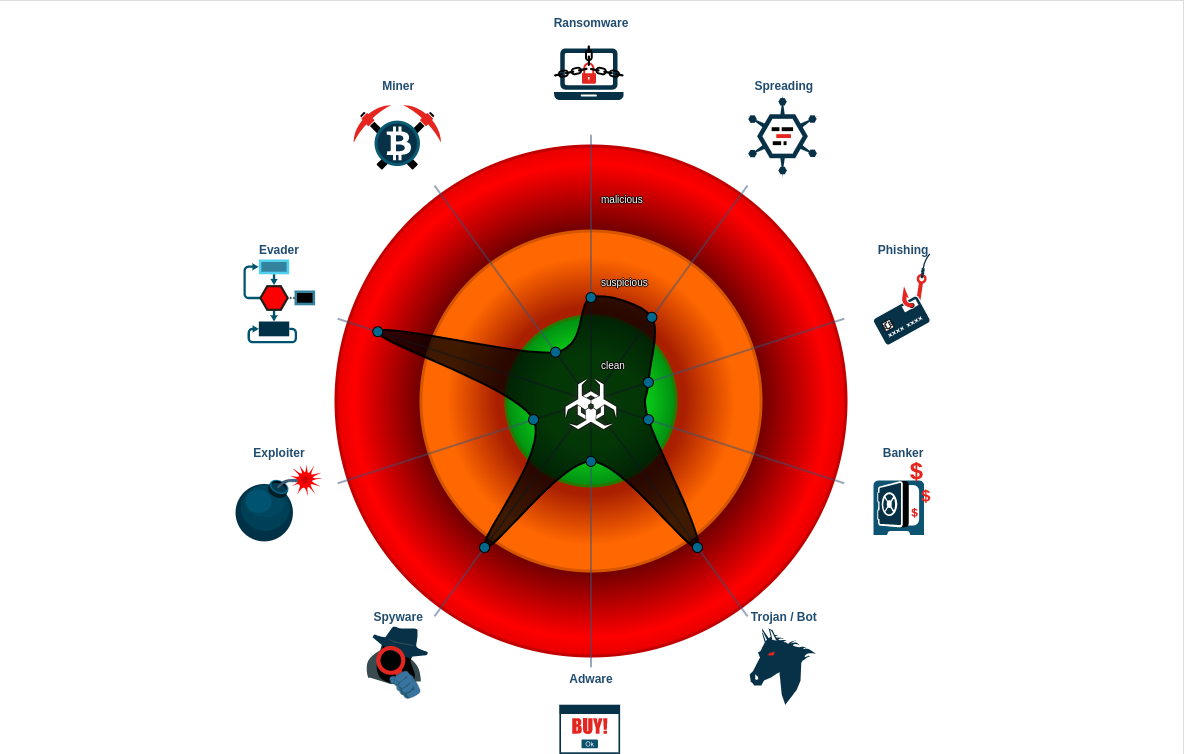
\includegraphics[scale=0.3]{ZEUS_CLASSIFICATION.png}


When messing with malware on your machine I figured I would either want 
to run it in a VM or make sure none of the prerequisites are enabled on
the machine itself. This is where malware written in C or C++ thrive as
languages like Python and Java need the run time and interpreter already
installed to meet that prerequisite. For this assignment I decided to
take a look at the Zeus Trojan malware pkg that initially gaining
traction in the late 2000s when used to steal info from the US DOT.
Trojans are known to be malware that behaves as legitimate programs. The
bot would go on to infecting millions of computers and spawning any
variants. The bot is aimed to target windows machines to extract banking
in formations using keystroke logging. This form of attack is a common
example of a man-in-the-middle attack. The malware pkg performs
infection via phishing schemes or drive-by downloads and infected some
of the largest companies such as Bank of America, Oracle, Cisco, Amazon,
etc. The Trojan violates just about every principle in the CIA triad.
Since confidential banking information was taken as well as money,
confidentially and integrity are both violated while availability
remains in questions. Patches to the malware offered from cybersecurity
consultants is known to eradicate it from the infected machine, however
strains of the virus were spawned remaining a constant battle.
I was able to find several versions of the "leaked" banking trojan but
check out the version I had found from here!

\url{https://github.com/touyachrist/evo-zeus}

Although not the most dentrimental part of the source code, in a repo
containing the Zeus source code this block minimally shows the entry
point to the windows core API was created and giving root permission

\begin{verbatim}

void WINAPI entryPoint(void) {
  Mem::init();
  Console::init();  
  Crypt::init();
  Core::init();
  
  CUI_DEFAULT_COMMANDLINE_HELPER;

  Core::uninit();
  Crypt::uninit();
  Console::uninit();
  Mem::uninit();
  
  CWA(kernel32, ExitProcess)(coreData.exitCode);
}

%\end{verbatim}

A similar version of this code I ran on my machine running kali linux, was 
able to give me root permissions as a regular user. 
See here (maybe it works for you):

\begin{verbatim}
int getuid(){
    return 0;
}
int geteuid(){
    return 0;
}
int getgid(){
    return 0;
}
int getegid(){
    return 0;
}
\end{verbatim}








\end{document}
